% *****************************************************************************
% CSG specific modification of the ClassicThesis style by André Mide.
% see https://ctan.org/pkg/classicthesis for more information on the original
% template!
%
% License:
% This program is free software; you can redistribute it and/or modify
% it under the terms of the GNU General Public License as published by
% the Free Software Foundation; either version 2 of the License, or
% (at your option) any later version.
%
% This program is distributed in the hope that it will be useful,
% but WITHOUT ANY WARRANTY; without even the implied warranty of
% MERCHANTABILITY or FITNESS FOR A PARTICULAR PURPOSE.  See the
% GNU General Public License for more details.
%
% You should have received a copy of the GNU General Public License
% along with this program; see the file COPYING.  If not, write to
% the Free Software Foundation, Inc., 59 Temple Place - Suite 330,
% Boston, MA 02111-1307, USA.
% *****************************************************************************
\RequirePackage{silence} % :-\
    \WarningFilter{scrreprt}{Usage of package `titlesec'}
    %\WarningFilter{scrreprt}{Activating an ugly workaround}
    \WarningFilter{titlesec}{Non standard sectioning command detected}
\documentclass[ twoside,openright,titlepage,numbers=noenddot,%1headlines,
                headinclude,footinclude,cleardoublepage=empty,abstract=on,
                BCOR=5mm,paper=a4,fontsize=11pt,dvipsnames
                ]{scrreprt}

% *****************************************************************************
% Note: Make all your adjustments in here
% *****************************************************************************
% *****************************************************************************
% 0. Set the encoding of your files. UTF-8 is the only sensible encoding
% nowadays. If you can't read äöüßáéçèê∂åëæƒÏ€ then change the encoding setting
% in your editor, not the line below. If your editor does not support utf8 use
% another editor!
% *****************************************************************************
\PassOptionsToPackage{utf8}{inputenc}
\usepackage{inputenc}

\PassOptionsToPackage{T1}{fontenc} % T2A for cyrillics
\usepackage{fontenc}

% *****************************************************************************
% Personal data and user ad-hoc commands (insert your own data here)
% *****************************************************************************
\newcommand{\myTitle}{Your Title Here\xspace}
\newcommand{\myName}{Your Name Here\xspace}
\newcommand{\myMatNr}{00000 \xspace}
\newcommand{\myPlaceOfBirth}{City, Country\xspace}
\newcommand{\myProf}{Holger Fröning\xspace}
\newcommand{\mySupervisor}{Jon Doe\xspace}
\newcommand{\myLocation}{Heidelberg\xspace}
\newcommand{\mySubmissionDate}{Day/Month/Year Here\xspace}
\newcommand{\myVersion}{\classicthesis}



% *****************************************************************************
% 1. Configure classicthesis for your needs here, e.g., remove "drafting" below
% in order to deactivate the time-stamp on the pages
% (see ClassicThesis.pdf for more information):
% *****************************************************************************
\PassOptionsToPackage{
	drafting=false,    % print version information on the bottom of the pages
	tocaligned=false, % the left column of the toc will be aligned (no indentation)
	dottedtoc=false,  % page numbers in ToC flushed right
	eulerchapternumbers=true, % use AMS Euler for chapter font (otherwise Palatino)
	linedheaders=false,       % chaper headers will have line above and beneath
	floatperchapter=true,     % numbering per chapter for all floats (i.e., Figure 1.1)
	eulermath=false,  % use awesome Euler fonts for mathematical formulae (only with pdfLaTeX)
	beramono=true,    % toggle a nice monospaced font (w/ bold)
	palatino=true,    % Use Palatino font
	style=arsclassica % classicthesis, arsclassica
}{classicthesis}


% *****************************************************************************
% 2. Setup, finetuning, and useful commands
% *****************************************************************************
\providecommand{\mLyX}{L\kern-.1667em\lower.25em\hbox{Y}\kern-.125emX\@}
\newcommand{\ie}{i.\,e.}
\newcommand{\Ie}{I.\,e.}
\newcommand{\eg}{e.\,g.}
\newcommand{\Eg}{E.\,g.}
\newcommand{\MatVal}[1]{\bm{\mathit{#1}}} % use to typeset matrix variables
% *****************************************************************************


% *****************************************************************************
% 3. Loading some handy packages
% *****************************************************************************
\PassOptionsToPackage{ngerman,american}{babel} % change this to your language(s), main language last
% Spanish languages need extra options in order to work with this template
%\PassOptionsToPackage{spanish,es-lcroman}{babel}
\usepackage{babel}

\usepackage{csquotes}
\PassOptionsToPackage{%
	backend=biber,bibencoding=utf8, %instead of bibtex
	% backend=bibtex8,bibencoding=ascii,%
	language=auto,%
	style=numeric-comp,%
	%style=authoryear-comp, % Author 1999, 2010
	%bibstyle=authoryear,dashed=false, % dashed: substitute rep. author with ---
	sorting=nyt, % name, year, title
	maxbibnames=10, % default: 3, et al.
	%backref=true,%
	natbib=true % natbib compatibility mode (\citep and \citet still work)
}{biblatex}
\usepackage{biblatex}

\PassOptionsToPackage{fleqn}{amsmath}       % math environments and more by the AMS
\usepackage{amsmath}

% *****************************************************************************
% General useful packages
% *****************************************************************************
\usepackage{verbatimbox}
\usepackage{bm}
\usepackage{mathdots}
\usepackage{mathtools}
\usepackage{tikz}
\usetikzlibrary{trees, matrix, positioning, patterns, shapes, shadows, shapes.arrows, arrows.meta, shapes.multipart, decorations.pathreplacing, calc, tikzmark, shapes.geometric}
\usepackage[binary-units]{siunitx}
\usepackage{lipsum}
\usepackage{graphicx} %
\usepackage{scrhack} % fix warnings when using KOMA with listings package
\usepackage{xspace} % to get the spacing after macros right
\PassOptionsToPackage{printonlyused,smaller}{acronym}
\usepackage{acronym} % nice macros for handling all acronyms in the thesis
\def\bflabel#1{{\acsfont{#1}\hfill}}
\def\aclabelfont#1{\acsfont{#1}}
% *****************************************************************************
\usepackage{pgfplots} % External TikZ/PGF support (thanks to Andreas Nautsch)
\pgfplotsset{compat=1.18}
\usepgfplotslibrary{units}
%\usetikzlibrary{external}
%\tikzexternalize[mode=list and make, prefix=ext-tikz/]
% *****************************************************************************


% *****************************************************************************
% 4. Setup floats: tables, (sub)figures, and captions
% *****************************************************************************
\usepackage{tabularx} % better tables
\setlength{\extrarowheight}{3pt} % increase table row height
\newcommand{\tableheadline}[1]{\multicolumn{1}{l}{\spacedlowsmallcaps{#1}}}
\newcommand{\myfloatalign}{\centering} % to be used with each float for alignment
\usepackage{subfig}
% *****************************************************************************


% *****************************************************************************
% 5. Setup code listings
% *****************************************************************************
\usepackage{listings}
%\lstset{emph={trueIndex,root},emphstyle=\color{BlueViolet}}%\underbar} % for special keywords
\lstset{language=C++,
	morekeywords={float2,float3,float4,__device__,__forceinline__,__host__,__global__},
	keywordstyle=\color{RoyalPurple},%\bfseries,
	basicstyle=\footnotesize\ttfamily,
	identifierstyle=\color{WildStrawberry},
	commentstyle=\color{SeaGreen}\ttfamily,
	stringstyle=\ttfamily,
	numbers=left,%left,%
	numberstyle=\scriptsize,%\tiny
	stepnumber=1,
	numbersep=8pt,
	showstringspaces=false,
	breaklines=true,
	%frameround=ftff,
	frame=single,
	belowcaptionskip=.75\baselineskip,
  captionpos=b
	%frame=L
}
% *****************************************************************************

\usepackage{classicthesis}

% *****************************************************************************
% Fine-tune hyperreferences (hyperref should be called last)
% *****************************************************************************
\hypersetup{%
	%draft, % hyperref's draft mode, for printing see below
	colorlinks=true, linktocpage=true, pdfstartpage=3, pdfstartview=FitV,%
	% uncomment the following line if you want to have black links (e.g., for printing)
	%colorlinks=false, linktocpage=false, pdfstartpage=3, pdfstartview=FitV, pdfborder={0 0 0},%
	breaklinks=true, pageanchor=true,%
	pdfpagemode=UseNone, %
	% pdfpagemode=UseOutlines,%
	plainpages=false, bookmarksnumbered, bookmarksopen=true, bookmarksopenlevel=1,%
	hypertexnames=true, pdfhighlight=/O,%nesting=true,%frenchlinks,%
	urlcolor=CTurl, linkcolor=CTlink, citecolor=CTcitation, %pagecolor=RoyalBlue,%
	%urlcolor=Black, linkcolor=Black, citecolor=Black, %pagecolor=Black,%
	pdftitle={\myTitle},%
	pdfauthor={\textcopyright\ \myName, Heidelberg University, Institute of Computer Engineering},%
	pdfsubject={},%
	pdfkeywords={},%
	pdfcreator={pdfLaTeX},%
	pdfproducer={LaTeX with hyperref and classicthesis}%
}


% *****************************************************************************
% Setup autoreferences (hyperref and babel)
% *****************************************************************************
% There are some issues regarding autorefnames
% http://www.tex.ac.uk/cgi-bin/texfaq2html?label=latexwords
% you have to redefine the macros for the
% language you use, e.g., american, ngerman
% (as chosen when loading babel/AtBeginDocument)
% *****************************************************************************
\makeatletter
\@ifpackageloaded{babel}%
{%
	\addto\extrasamerican{%
		\renewcommand*{\figureautorefname}{Figure}%
		\renewcommand*{\tableautorefname}{Table}%
		\renewcommand*{\partautorefname}{Part}%
		\renewcommand*{\chapterautorefname}{Chapter}%
		\renewcommand*{\sectionautorefname}{Section}%
		\renewcommand*{\subsectionautorefname}{Section}%
		\renewcommand*{\subsubsectionautorefname}{Section}%
	}%
	\addto\extrasngerman{%
		\renewcommand*{\paragraphautorefname}{Absatz}%
		\renewcommand*{\subparagraphautorefname}{Unterabsatz}%
		\renewcommand*{\footnoteautorefname}{Fu\"snote}%
		\renewcommand*{\FancyVerbLineautorefname}{Zeile}%
		\renewcommand*{\theoremautorefname}{Theorem}%
		\renewcommand*{\appendixautorefname}{Anhang}%
		\renewcommand*{\equationautorefname}{Gleichung}%
		\renewcommand*{\itemautorefname}{Punkt}%
	}%
	% Fix to getting autorefs for subfigures right (thanks to Belinda Vogt for changing the definition)
	\providecommand{\subfigureautorefname}{\figureautorefname}%
}{\relax}
\makeatother

\listfiles


% *****************************************************************************
% Bibliographies
% *****************************************************************************
\addbibresource{Bibliography.bib}

% *****************************************************************************
% Contents
% *****************************************************************************
\begin{document}
\frenchspacing
\raggedbottom
\selectlanguage{american} % american ngerman
%\renewcommand*{\bibname}{new name}
%\setbibpreamble{}
\pagenumbering{roman}
\pagestyle{plain}
% *****************************************************************************
% Frontmatter
% *****************************************************************************
% Choose appropriate Titlepage below if you choose the DACS version, also
% comment line 92 - DeclarationTI
% Dirty Title
\thispagestyle{empty}
\begin{addmargin}[-1cm]{-3cm}
	\begin{center}
		\begingroup
		\Huge Faculty of Engineering Sciences \\ \medskip
		\endgroup

		\begingroup
		\Large Heidelberg University \\ \bigskip
		\endgroup

		\hfill
		\vfill

		\begingroup
    \Large
		Master Thesis \\
		in Computer Engineering \\
		submitted by \\
		\myName \\
		born in \myPlaceOfBirth \\
		\mySubmissionDate
		\endgroup
	\end{center}
\end{addmargin}

% Actual Title
\begin{titlepage}
\begin{addmargin}[-1cm]{-3cm}
	\begin{center}
		\large
		\begingroup
		\huge
		\spacedallcaps{\myTitle} \\ \bigskip
		\endgroup
		\vfill
		\hfill

		This Master thesis has been carried out by \myName \\
		at the \\
		Institute of Computer Engineering \\
		under the supervision of \\
		\myProf
	\end{center}
\end{addmargin}
\end{titlepage}

% \begin{titlepage}
\begin{addmargin}[-1cm]{-3cm}
	\begin{center}
		\begingroup
		\Huge
		Heidelberg University \\ \bigskip
		\endgroup

		\begingroup
		\Large
		Institute of Computer Engineering \\ \smallskip
		\endgroup

		\begingroup
		\Large
		Computing Systems Group \\ \smallskip
		\endgroup

		\begingroup
		\Large
		Master's Thesis \\ \bigskip
		\endgroup

		\begingroup
		\Huge
		\myThesisTitle \\ \smallskip
		\endgroup

		\vfill
		\hfill
	\end{center}
	\begingroup
	\large
	\noindent
	\begin{tabular}{ll}
		Name: & \myName \\
		Matriculation number: & \myMatNr \\
		Supervisor: & \myProf \\
		Date of submission: & \myThesisSubmissionDate \\
	\end{tabular}
	\endgroup
\end{addmargin}
\end{titlepage}
\cleardoublepage

\pdfbookmark[0]{Declaration}{declaration}
\chapter*{Declaration}
\thispagestyle{empty}
I hereby certify that I have written the work myself and that I have not used
any sources or aids other than those specified and that I have marked what
has been taken over from other people's works, either verbatim or in terms of
content, as foreign. I also certify that the electronic version of my thesis
transmitted completely corresponds in content and wording to the printed
version. I agree that this electronic version is being checked for plagiarism
at the university using plagiarism software.
\bigskip

\noindent\textit{Heidelberg, \myThesisSubmissionDate}

\smallskip

\begin{flushright}
	\begin{tabular}{m{5cm}}
		\\ \hline
		\centering\myName \\
	\end{tabular}
\end{flushright}

% \begin{titlepage}
\begin{addmargin}[-1cm]{-3cm}
	\begin{center}
		\begingroup
		\Huge
		Project Report \\ \bigskip
		\endgroup

		\begingroup
		\Large
		Computing Systems Group \\ \smallskip
		\endgroup

		\begingroup
		\Huge
		\myTitle \\ \smallskip
		\endgroup

		\vfill
		\hfill
	\end{center}
	\begingroup
	\large
	\noindent
	\begin{tabular}{ll}
		Name: & \myName \\
		Supervisor: & \mySupervisor \\
		Date of submission: & \mySubmissionDate \\
	\end{tabular}
	\endgroup
\end{addmargin}
\end{titlepage}
\cleardoublepage

\cleardoublepage\pdfbookmark[1]{Abstract}{Abstract}
\begingroup
\let\clearpage\relax
\let\cleardoublepage\relax
\let\cleardoublepage\relax

% English version

\chapter*{Abstract}

% Briefly summarize the contents of your work in 150-250 words.
% \lipsum[1]
% The boom in usage of ML applications goes hand in hand with a boom in its energy costs. This necessitates a better understanding of present and future ML performance characteristics. No previous work has profiled both time and energy for inference and training while providing predictions for unknown operations. We therefore contribute a pipeline to profile all four cases and a model to predict all of them. Lastly we contribute detailed results and validations, along with obervations on general trends for optimally efficient execution. We provide a tool enabling the correct choice of target GPU and clock speed for existing and future models.



% The fast broader adoption of ML applications has caused a surge in energy requirements, necessitating a better understanding of the tradeoffs between time and energy for ML performance. Previous work was focused on time-only or inference-only studies. We contribute: (1) time and energy profiling across inference and training, (2) performance prediction trained on our profiling results and (3) graphical evalutation and validation of profiling and predictor results. Profiling results of A30 performance across several core clocks reveal an energy optimum of 900 MHz, aligning with the manufacturer base clock of 930 MHz. This work provides the tools, which enable the correct choice of target GPU and clock speed for existing and future models.


% increase in parameter count 

% tradeoffs between execution speed and energy consumption

% tradeoffs between execution speed and energy costs


% time and energy profiling across inference and training of DNN operations 


% % has caused a surge in their global energy usage


% operations-level and full DNN performance prediction


The fast broader adoption of ML applications has caused a surge in their global energy usage, necessitating a comprehensive understanding of the tradeoffs between execution speed and energy consumption. While previous work was focused on time-only or inference-only studies, we provide a more complete picture by covering a wider space of parameters. We contribute: (1) time and energy profiling across inference and training of DNN operations, (2) operations-level and full DNN performance predictions trained on our profiling results and (3) graphical evaluation and validation of profiling and predictor results. Profiling results of Nvidia A30 performance across several core clocks reveal an energy optimum of 900 MHz, aligning with the manufacturer base clock of 930 MHz. This work provides the tools which enable the correct choice of target GPU and clock speed for existing and future models.



% The fast broader adoption of ML applications has caused a surge in their energy requirements, necessitating a comprehensive understanding of the tradeoffs and costs. While previous work was focused on time-only or inference-only studies, we provide a more complete picture by covering a wider space of parameters. We contribute: (1) time and energy profiling across inference and training, (2) performance prediction trained on our profiling results and (3) graphical evaluation and validation of profiling and predictor results. Profiling results of Nvidia A30 performance across several core clocks reveal an energy optimum of 900 MHz, aligning with the manufacturer base clock of 930 MHz. This work provides the tools which enable the correct choice of target GPU and clock speed for existing and future models.



\newpage

% German version

\begin{otherlanguage}{ngerman}
\pdfbookmark[1]{Zusammenfassung}{Zusammenfassung}
\chapter*{Zusammenfassung}

% Die rasche Verbreitung von ML Anwendungen hat zu einem starken Anstieg der Energiekosten geführt und damit ein besseres Verständnis der 
% Tradeoffs zwischen Zeit und Energie notwendig gemacht. Der Fokus vorheriger Arbeiten liegt auf reinen Zeit oder reinen Inference Studien. Unsere Contributions sind: (1) Zeit- und Energieprofiling für Inference und Training, (2) Vorhersagen trainiert auf den Profiling Ergebnissen und (3) eine grafische Auswertung und Validierung der Profiling und Verhersage Ergebnisse. Messresultate der A30 Performance über einige GPU Clocks zeigen ein Energieoptimum bei 900 MHz, welches sich mit dem Standard Base Clock von 930 MHz deckt. Diese Arbeit gibt uns die Werkzeuge um die richtige GPU und den richtigen Clock Speed für aktuelle und zuküftige Modelle zu wählen.


Die rasche Verbreitung von ML Anwendungen hat zu einem starken Anstieg ihrer globalen Energiekosten geführt und damit ein umfassendes Verständnis der Tradeoffs zwischen Laufzeit und Energieverbrauch notwendig gemacht. Der Fokus vorheriger Arbeiten liegt auf reinen Zeit- oder reinen Inference-Studien. Hierauf bauen wir auf, indem wir eine breitere Spanne an Parametern abdecken um ein vollständigeres Bild der Lage abzugeben. Unsere Contributions sind: (1) Zeit- und Energieprofiling für Inference und Training von DNN Operations, (2) Vorhersagen für individuelle Operations und volle DNNs trainiert auf den Profiling Ergebnissen und (3) eine grafische Auswertung und Validierung der Profiling und Vorhersage Ergebnisse. Messresultate der Nvidia A30 Performance über einige GPU Clocks zeigen ein Energieoptimum bei 900 MHz, welches sich mit dem Standard Base Clock von 930 MHz deckt. Diese Arbeit stellt die Werkzeuge zur Verfügung um die richtige GPU und den richtigen Clock Speed für aktuelle und zukünftige Modelle zu wählen.
\end{otherlanguage}

\endgroup

\vfill

% Comment line below to skip Acknowledgments
\cleardoublepage\pdfbookmark[1]{Acknowledgments}{acknowledgments}

%Optional qote, comment or delete to skip
% \begin{flushright}{\slshape
% 		Nice quote here.} \\ \medskip
% 	--- Some Author
% \end{flushright}



\bigskip

\begingroup
\let\clearpage\relax
\let\cleardoublepage\relax
\let\cleardoublepage\relax
\chapter*{Acknowledgments}

I would like to express my gratitude to Daniel Barley for his dedicated guidance and insightful feedback throughout this thesis. My thanks also go to the sig-profiling group for fostering a collaborative research environment. Additionally, I am grateful to Alexandra Stehle for her early input, as well as to Mathias Backes, Marlene Matzke, and Alexander Seitz for their feedback and support.

\endgroup

\cleardoublepage\pagestyle{scrheadings}
\pdfbookmark[1]{\contentsname}{tableofcontents}
\setcounter{tocdepth}{2} % <-- 2 includes up to subsections in the ToC
\setcounter{secnumdepth}{3} % <-- 3 numbers up to subsubsections
\manualmark
\markboth{\spacedlowsmallcaps{\contentsname}}{\spacedlowsmallcaps{\contentsname}}
\tableofcontents
\automark[section]{chapter}
\renewcommand{\chaptermark}[1]{\markboth{\spacedlowsmallcaps{#1}}{\spacedlowsmallcaps{#1}}}
\renewcommand{\sectionmark}[1]{\markright{\textsc{\thesection}\enspace\spacedlowsmallcaps{#1}}}

% *****************************************************************************
% Mainmatter
% *****************************************************************************
\cleardoublepage
\pagestyle{scrheadings}
\pagenumbering{arabic}
% use \cleardoublepage here to avoid problems with pdfbookmark
\chapter{Scientific Article}
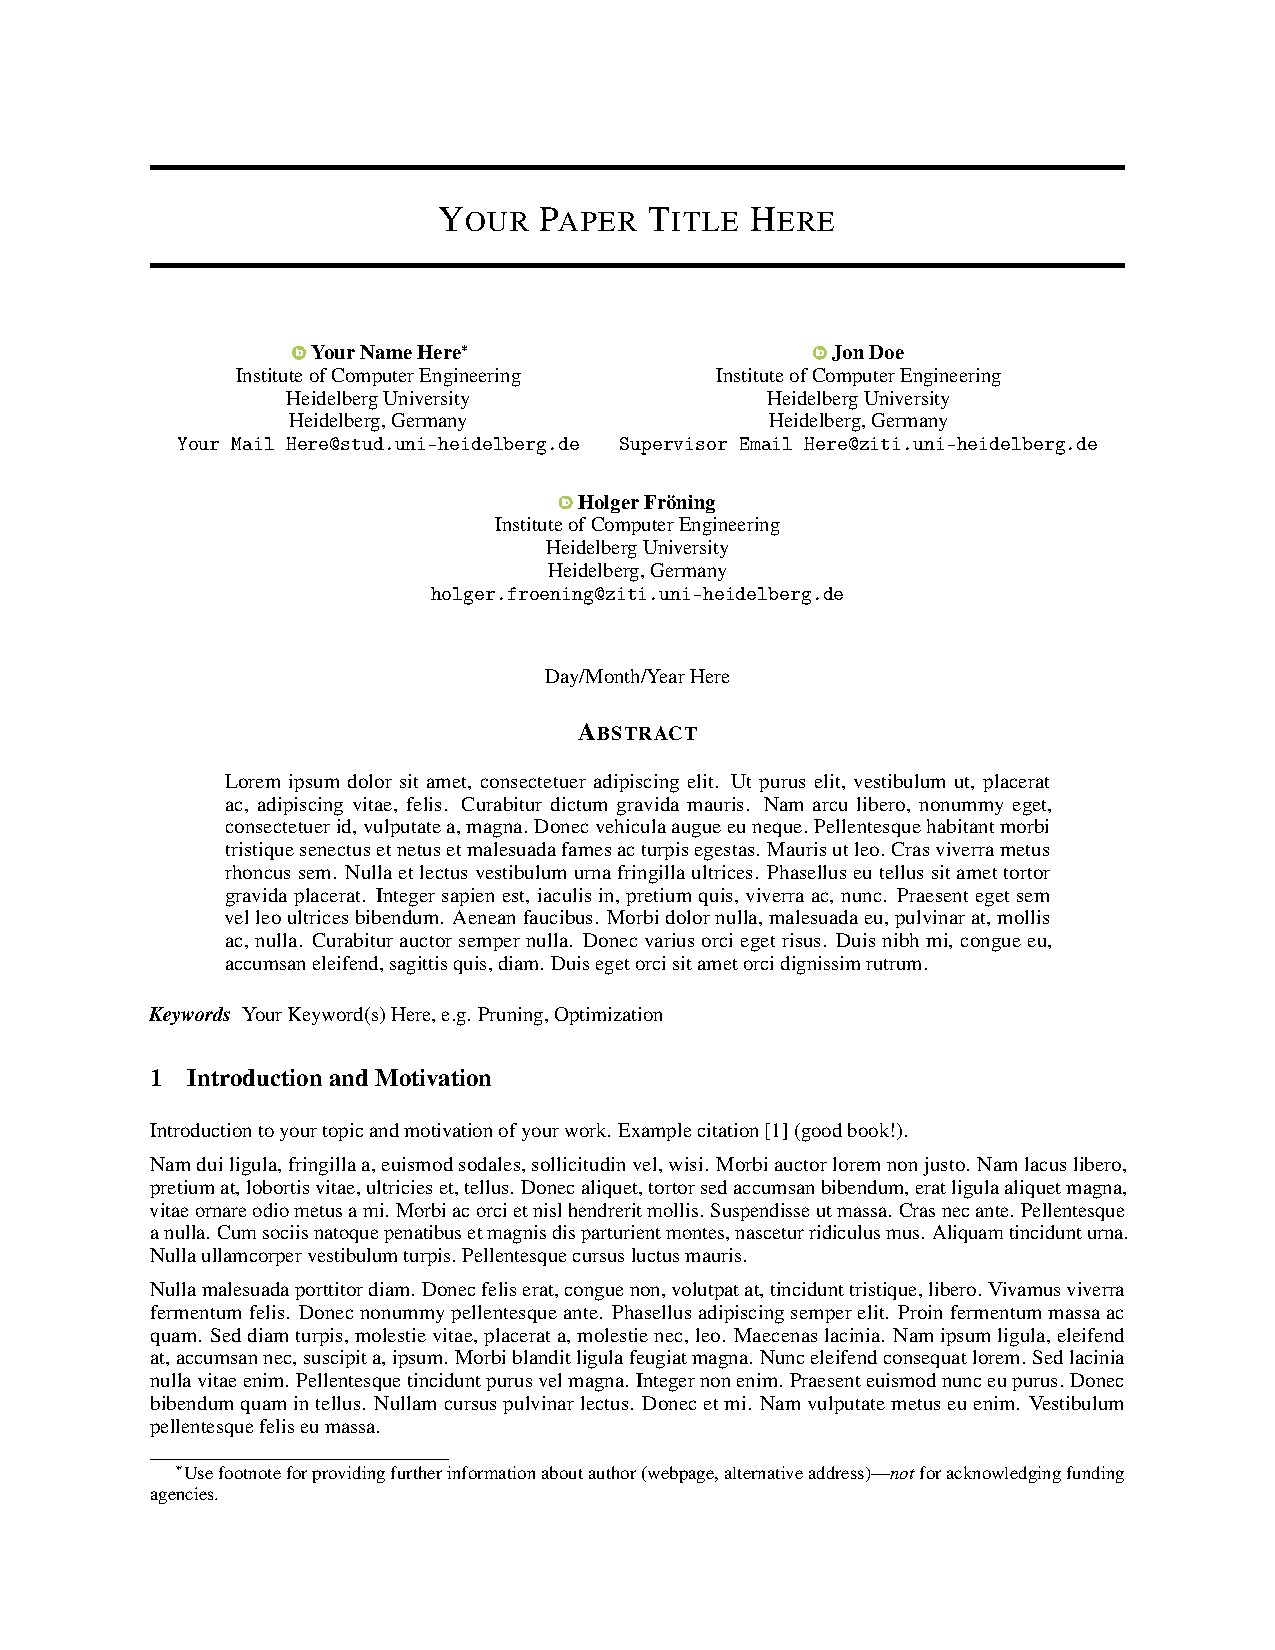
\includepdf[
	pages=-
	addtotoc={
		1, section, 1, Introduction and Motivation, sec:introduction
	}
]{PaperThesis}
\cleardoublepage
% *****************************************************************************
% Backmatter
% *****************************************************************************
\appendix
\renewcommand{\thechapter}{\alph{chapter}}
\chapter{Appendix}
Appendix here
\section{test}
A section

\cleardoublepage
\chapter{Implementation}

Provide technical details of your implementation here.

\cleardoublepage
\chapter{Evaluation}

Extended description of you experimental setup and supplementary results here.

\cleardoublepage
\chapter{Discussion and Outlook}

Give and extended discussion and outlook of your work here.

% *****************************************************************************
% Other Stuff in the Back
% *****************************************************************************
\cleardoublepage%********************************************************************
% Bibliography
%*******************************************************
% work-around to have small caps also here in the headline
% https://tex.stackexchange.com/questions/188126/wrong-header-in-bibliography-classicthesis
% Thanks to Enrico Gregorio
\defbibheading{bibintoc}[\bibname]{%
  \phantomsection
  \manualmark
  \markboth{\spacedlowsmallcaps{#1}}{\spacedlowsmallcaps{#1}}%
  \addtocontents{toc}{\protect\vspace{\beforebibskip}}%
  \addcontentsline{toc}{chapter}{\tocEntry{#1}}%
  \chapter*{#1}%
}
\printbibliography[heading=bibintoc]

\cleardoublepage%*******************************************************
% Declaration
%*******************************************************
\begin{otherlanguage}{ngerman}
\pdfbookmark[0]{Declaration}{declaration}
\chapter*{Erklärung}
\thispagestyle{empty}
Folgende Teile der Arbeit wurden gemeinschaftlich durch Supervisor hier,
Herrn Holger Fröning und mich erstellt:

\begin{itemize}
     \item das zugrundeliegende Konzept,
     \item der wissenschaftliche Artikel (Teil A. der Arbeit). 
\end{itemize}

Alle anderen Teile wurden von mir selbständig und nur unter Zuhilfenahme der
angegebenen Quellen und Hilfsmittel erstellt. Im Detail sind dies:

\begin{itemize}
     \item die gesamte Implementierung,
     \item alle durchgeführten Experimente,
     \item sowie der Appendix (Teil II. der Arbeit).
\end{itemize}

Dabei habe ich die Grundsätze und Empfehlungen „Verantwortung in der
Wissenschaft“ der Universität Heidelberg beachtet. Ferner versichere ich,
dass die abgegebene digitale Version mit der gedruckten Version
übereinstimmen.

\bigskip

\noindent\textit{Heidelberg, den \myThesisSubmissionDate}

\smallskip

\begin{flushright}
    \begin{tabular}{m{5cm}}
        \\ \hline
        \centering\myName \\
    \end{tabular}
\end{flushright}
\end{otherlanguage}

\end{document}
% *****************************************************************************
